\documentclass[11pt,a4paper]{article}
\usepackage[T1]{fontenc}\usepackage[utf8]{inputenc}\usepackage[scaled=0.95]{helvet}\renewcommand{\familydefault}{\sfdefault}
\usepackage[a4paper,margin=2.2cm]{geometry}\usepackage{graphicx,booktabs,longtable,amsmath,caption,xcolor,enumitem,array,float}\usepackage[hidelinks]{hyperref}
\captionsetup{font=small,labelfont=bf}\setlength{\parskip}{0.55em}\setlength{\parindent}{0pt}\setlist{itemsep=0.25em,topsep=0.3em}\widowpenalty=10000\clubpenalty=10000\raggedbottom
\newcommand{\docversion}{2026-11-10-11-16-01}
\begin{document}
{\raggedright\LARGE\bfseries Weather, daylight, snow and bicycle traffic on rue de Terrebonne\par}\vspace{0.3em}
{\large Six count series, August 2024 to November 2026\par}\vspace{0.6em}
{\small Terrebonne-open-sources, version \docversion. Author: Rick Hoge, PhD (see the repository\textquoteright{}s « About the author »). Scripts, tables and figures: \url{https://github.com/OpenMobilityData/Terrebonne-open-sources/tree/main/2026-weather-and-bike-traffic}.\par}
\begin{center}\colorbox{red!15}{\parbox{0.96\textwidth}{\centering\textbf{\textcolor{red!70!black}{DRAFT for the author\textquoteright{}s review, November 10, 2026. Not yet checked line by line; figures may change.}}}}\end{center}
\subsection*{Lay summary}
How much does weather change cycling on rue de Terrebonne? This note uses every count available: citizen-operated camera sensors at King Edward and Draper, the borough\textquoteright{}s counter at Kensington, the City\textquoteright{}s detector at Girouard, and trips at the BIXI station at Grand Boulevard. Weather is from Trudeau airport; counts run August 2024 to November 2026.

Temperature matters most. Each degree warmer brings 5 to 6 per cent more bicycles, up to about 20 $^\circ$C, then levels off. A day at 0 $^\circ$C sees 30 to 43 per cent of the bicycles of the same day at 20 $^\circ$C; a day at $-$10 $^\circ$C, 17 to 28 per cent. There is no temperature below which cycling stops.

A day with 2 to 10 mm of rain has 14 to 22 per cent fewer bicycles than a dry day at the same temperature; snow on the ground goes with 31 to 47 per cent fewer at three of the four counters. At the same evening hour and temperature, the borough\textquoteright{}s counter records 27 per cent fewer bicycles after sunset.

Cold, snow and short days arrive together, so much of the winter drop could be either weather or season. Snow-loading days look like other winter days, but are too few to be sure. Year to year, with each year\textquoteright{}s weather accounted for, the result depends on the location: the west-end camera (King Edward) counted 27 per cent more in autumn 2026 than in its first year, the camera further east (Draper) 12 per cent fewer. The analysis accounts for sensor downtime (only complete days, compared like with like), but two to three years of counts cannot show whether cycling on the street is rising or falling.

Counters differ in place and type; only percentage changes are compared. The note makes no recommendation.
\subsection*{Abstract}
This note measures how the number of bicycles counted on rue de Terrebonne varies with the weather, with daylight and with snow, using every count series available for the street: two citizen-operated Telraam camera sensors (King Edward, 691 valid days from August 16, 2024; Draper, 509 days), the borough\textquoteright{}s loop counter at Kensington (284 days, eastbound, hourly release of June~4, 2026), the City\textquoteright{}s detector at Girouard (296 days, westbound), trips at the BIXI station on the street, and, as a reference, twelve City counters elsewhere in Montréal. Weather is Environment and Climate Change Canada\textquoteright{}s record at Montréal-Trudeau. Each series is modelled separately by negative binomial regression, so that every effect is a percentage and no levels are compared between series; the Telraam sensors, which count only in daylight, are analysed in a fixed window (08:00--16:00) that is daylight all year. The analysis accounts for sensor downtime: only days with a complete, valid count are used, no gap is filled in, and every comparison is between days of the same time of year, day type and weather, so that a period without data removes days from a comparison without being read as a drop in cycling. From one year to the next, with each year\textquoteright{}s weather taken into account in the model (a colder or snowier year is compared with what that weather predicts), the result depends on the location (King Edward, at the west end, +27\,\% (+12 to +45) in the autumn of 2026 against its first year; Draper, further east, $-$12\,\% ($-$20 to $-$5) after its first year), and two to three years of data do not establish a trend at either. Location is a parameter of every model: each counter is analysed as its own point on the street. The note states what was measured, with intervals, and what the data cannot show. It makes no recommendation.
\subsection*{What the analysis finds}
\begin{enumerate}
\item \textbf{Temperature.} On the four Terrebonne count series, each additional degree of daytime temperature goes with 5 to 6\,\% more bicycles, up to roughly 20\,$^\circ$C; above that the count stops rising. Holding rain, snow, wind, day of the week and time of year fixed, a day at 0\,$^\circ$C has 30 to 43\,\% of the count of the same day at 20\,$^\circ$C, and a day at $-$10\,$^\circ$C has 17 to 28\,\%. The count falls steadily with the cold; it does not fall to zero.
\item \textbf{No threshold in the cold.} In percentage terms the slope below 0\,$^\circ$C is not distinguishable from the slope between 0\,$^\circ$C and 20\,$^\circ$C on any Terrebonne series. The change of slope that the earlier analyses placed near $-$1 or $-$5\,$^\circ$C belongs to a straight-line model of the counts themselves; the only change of slope the data support is the levelling-off in warm weather, and its position is poorly determined (intervals of ten degrees or more).
\item \textbf{Wind chill.} Replacing air temperature and wind by the wind-chill index fits about as well (the two are correlated at 0.996); the data cannot separate them.
\item \textbf{Rain and snow.} At a given temperature and time of year, a day with 2 to 10\,mm of rain has 14 to 22\,\% fewer bicycles on the Terrebonne series, a day with more than 10\,mm 25 to 46\,\% fewer, and a day with at least 1\,cm of snow on the ground 31 to 47\,\% fewer at King Edward, Draper and Kensington, where it is the largest single weather effect after temperature; at the Girouard detector snow on the ground shows no measurable effect ($-$4 ($-$15 to +9)\,\%).
\item \textbf{Season or weather?} The two cannot be fully separated: 65 to 82\,\% of the day-to-day variation on the Terrebonne series can be attributed to either. Weather effects estimated only from the variation inside each calendar month are nonetheless close to those estimated over the whole record.
\item \textbf{Darkness.} On the loop counter, the same clock hour in the evening carries 27\,\% (19 to 34) fewer bicycles when the sun has set than when it is up, at the same temperature and in the same month.
\item \textbf{Snow loading.} On the days the City loaded snow in the sector that contains each counter, the counts are not distinguishable from other winter days once temperature and snow are accounted for; the intervals are wide (18 to 44 loading days per series).
\item \textbf{By location.} The counters stand at different points of the street, from King Edward at the west end (6.7\,km from downtown) to Girouard at the east end (4.9\,km), and each is analysed as its own location; a difference between two of them is a difference between places, and between instruments, not a discrepancy. The response to temperature is similar along the street (from 6.1\,\% per degree at King Edward to 4.6\,\% at Girouard); the effects of light rain, heavy rain, snow on the ground and the weekend do differ by location (tests in Section~\ref{sec:location}). On the days both camera sensors were valid, Draper counted 1.22 times what King Edward counted (1.16 to 1.29), the one comparison between two locations made with the same instrument.
\item \textbf{Year to year.} The weather of each year is part of the comparison: the model that estimates the difference between years also contains temperature, rain, snowfall, snow on the ground and wind, so a colder or snowier year is not mistaken for a decline. On that basis King Edward counted $-$1\,\% ($-$11 to +9) in its second counting year (from August~15, 2025) compared with its first, and +27\,\% (+12 to +45) from August~15 to November~8, 2026 compared with its first year. (compared plainly on the same dates, without the weather, $-$5 ($-$16 to +4)\,\% and +26 ($-$1 to +62)\,\%; its second year was colder and much snowier than its first). Draper counted $-$12\,\% ($-$20 to $-$5) after its first year, the BIXI station $-$10\,\% ($-$16 to $-$4), and the City\textquoteright{}s counters elsewhere $-$7\,\% ($-$14 to 0). The year-to-year figures are specific to each location and are not expected to be the same along the street. Downtime is accounted for in these figures: only days with a complete, valid count enter, and each is compared with days of the same time of year, day type and weather, so a gap in one year is not counted as a decline. The comparisons remain limited for other reasons: two to three years of data, a camera sensor whose field of view can change when it is remounted, and a third year that so far holds a single autumn. A year term absorbs every difference between the years other than the weather.
\end{enumerate}
\begin{figure}[p]\centering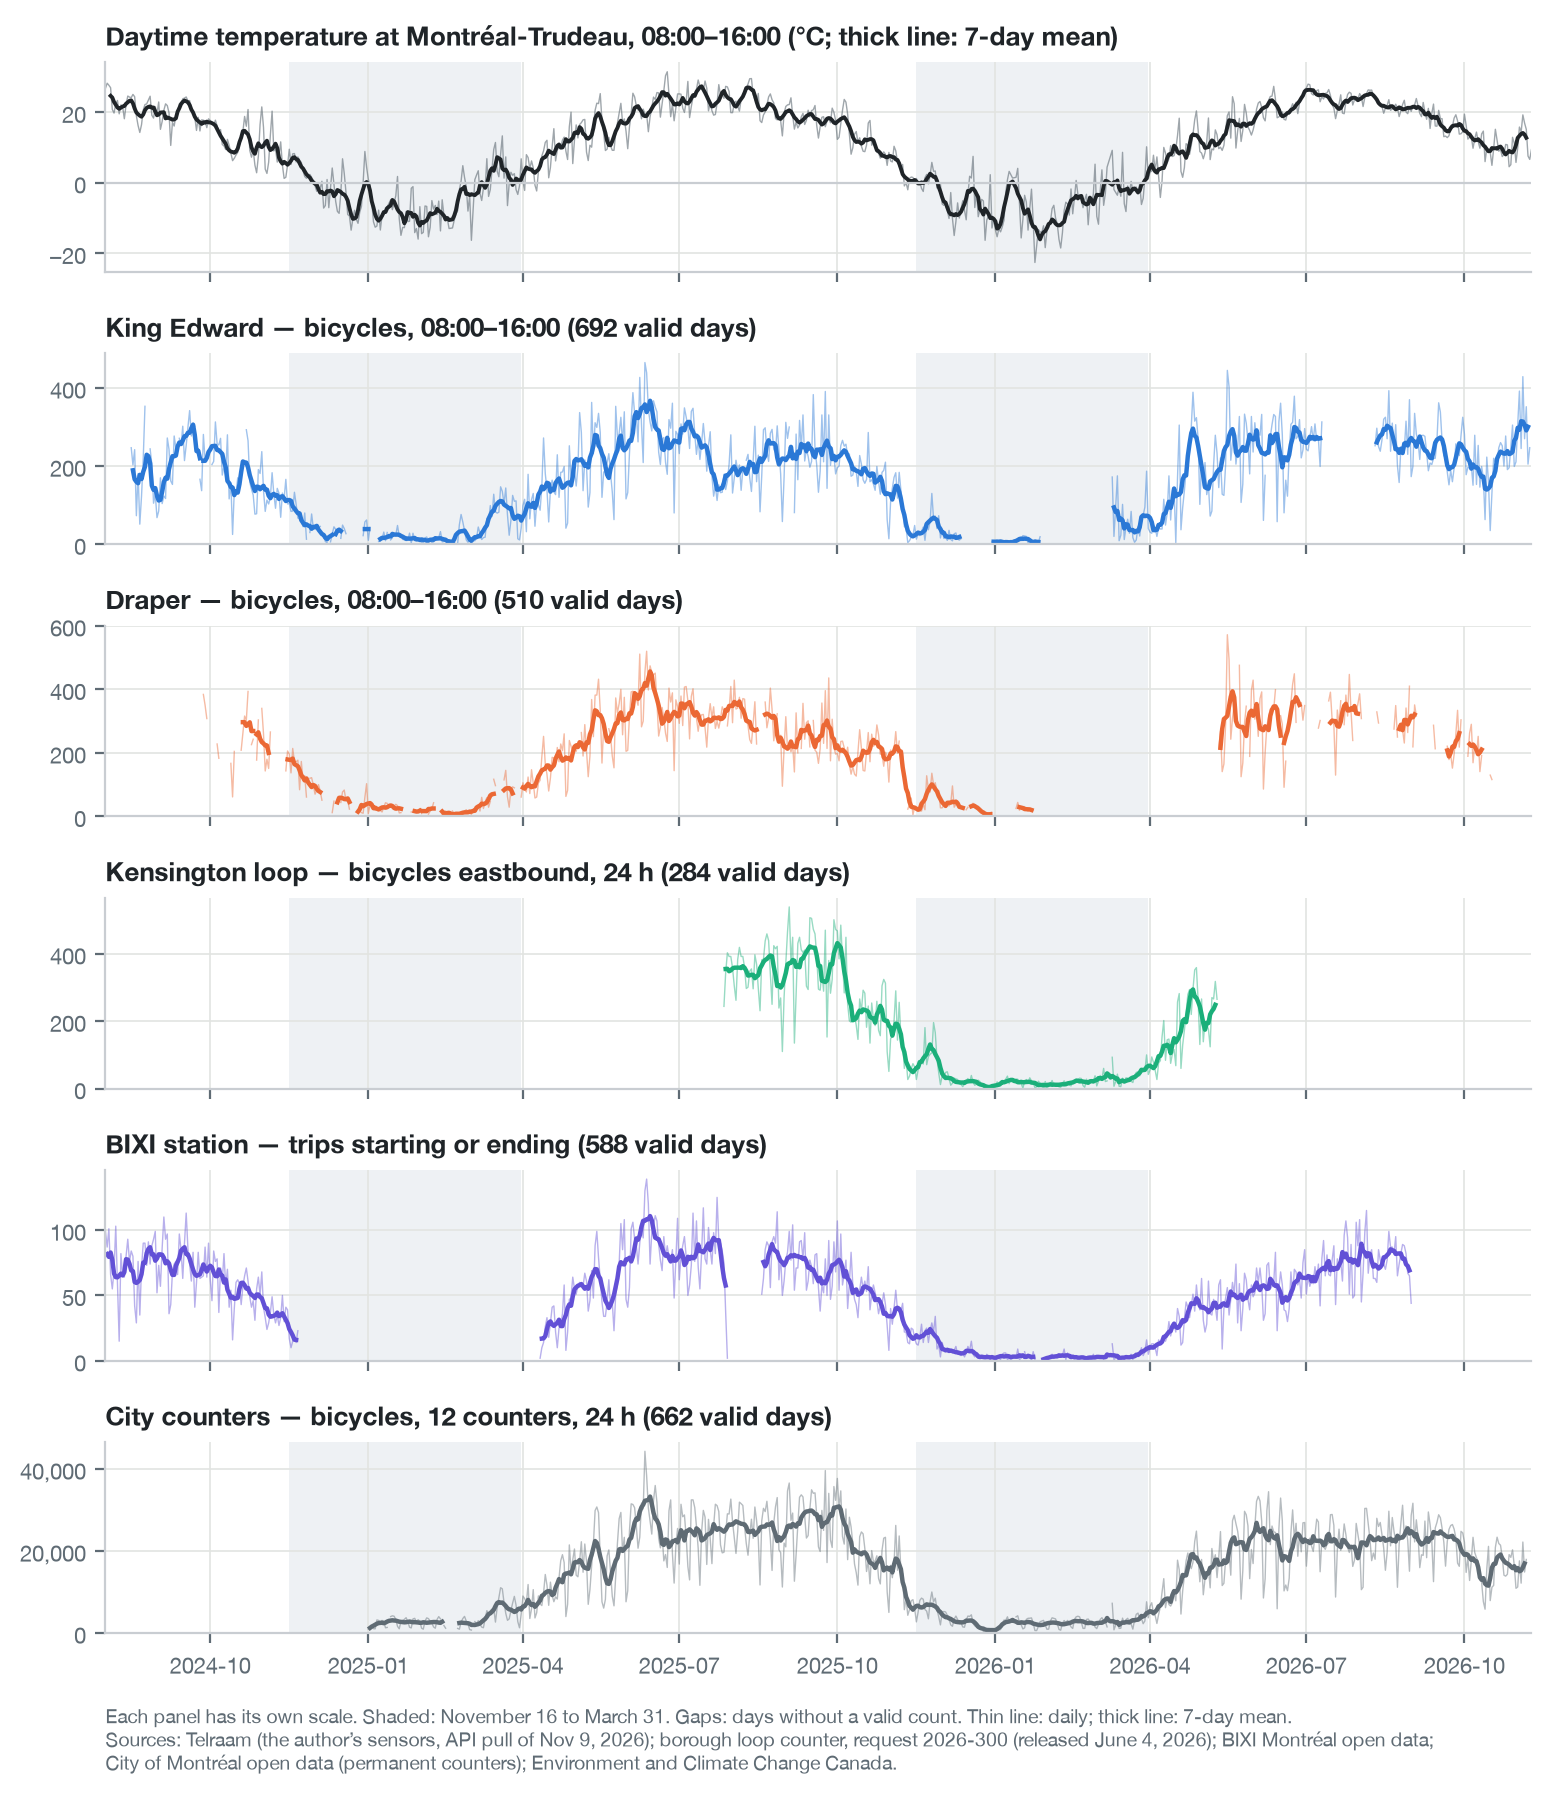
\includegraphics[width=0.97\textwidth]{../derived/figures/overview/overview_en.png}\caption{Daytime temperature and the daily count of each series. Each panel has its own scale; the series are not compared in level.}\label{fig:overview}\end{figure}
\tableofcontents\clearpage

\section{Questions}
\begin{enumerate}
\item How does the daily count of bicycles vary with temperature, and is there a temperature at which the response changes?
\item Does wind chill describe the response better than air temperature?
\item What do rain, snowfall, snow on the ground and wind each add at a given temperature?
\item How much of the seasonal swing can be attributed to weather, and how much to day length and the calendar?
\item Does a snowfall depress the counts on the following days, and do the days on which the City loads snow differ from other winter days?
\item How do the responses differ from one location on the street to another?
\item After weather is accounted for, does the count differ from one year to the next?
\end{enumerate}

\section{Data}
\subsection{The count series}
\begin{center}\small\begin{tabular}{@{}p{2.4cm}p{6.1cm}p{4.0cm}rr@{}}\toprule
Series & What is counted & Days used in the models & Days & Mean a day\\\midrule
King Edward & Bicycles, both directions, 08:00--16:00 (Telraam S2 camera sensor, west of Cavendish) & August 16, 2024 to November 8, 2026 & 691 & 163 \\
Kensington loop & Bicycles eastbound, 24 h (the borough\textquoteright{}s Eco-Counter loop) & July 27, 2025 to May 10, 2026 & 284 & 157 \\
Draper & Bicycles, both directions, 08:00--16:00 (Telraam S2 camera sensor, east of Cavendish) & September 25, 2024 to October 21, 2026 & 509 & 198 \\
Girouard detector & Bicycles westbound, 24 h (the City\textquoteright{}s pole-mounted detector at Girouard) & October 24, 2025 to October 15, 2026 & 296 & 121 \\
BIXI station & Trips starting or ending at the station « Grand Boulevard / de Terrebonne », April 15 to November 15 & August 2, 2024 to August 31, 2026 & 441 & 63 \\
City counters & Bicycles, 24 h, sum of twelve City loop counters elsewhere in Montréal & January 1, 2025 to November 6, 2026 & 661 & 14,821 \\
\bottomrule\end{tabular}\end{center}
The means are given to describe each series, not to compare them: a camera sensor counting eight daytime hours in both directions, one direction of a loop counting 24 hours, and trips at a bike-share dock are different quantities.

\textbf{Telraam sensors (King Edward, Draper).} Installed by Terrebonne residents in August and September 2024; the author was tasked with the statistical analysis of their data. Hourly counts from the Telraam API (pull of November~9, 2026). A Telraam sensor counts only in daylight. Its daily total therefore covers about nine hours in December and sixteen in June, and would rise and fall with the length of the day even if nobody changed their habits (Figure~\ref{fig:daylight}, left). To remove that artefact every analysis here uses the count in a \emph{fixed clock window, 08:00 to 16:00}, which is daylight on every day of the year at Montréal\textquoteright{}s latitude (the latest sunrise is about 07:35 and the earliest sunset about 16:10). The price is that the evening peak is left out. A day is valid when the sensor reported at least 8 hours with at least 6 hours of summed uptime, and all eight window hours with an uptime of at least 0.5. Invalid days are left out and nothing is interpolated. King Edward has no valid day in February 2026; Draper has none from February to April 2026 (Appendix~\ref{app:coverage}). Whether the API\textquoteright{}s hourly counts are already scaled for uptime could not be confirmed from Telraam\textquoteright{}s documentation; they are used as delivered.

\textbf{Kensington loop.} The borough\textquoteright{}s Eco-Counter (inductive loops, 24 hours, by direction). The hourly workbook released on June~4, 2026 under access request 2026-300 runs from July~26, 2025 to May~11, 2026. The westbound channel under-counts from about March~1, 2026, so the models use the eastbound channel alone. The daily table released on October~9, 2026 under request 2026-581 serves to identify the days set aside (May~29--31, 2026, zeros; June~7--9, 2026). One site, less than one full year, one direction.

\textbf{Girouard detector.} The City\textquoteright{}s pole-mounted detector at the corner of Girouard (open data « Compteurs cyclistes permanents », instance det-00118-01; files downloaded October~16, 2026) counts bicycles on Terrebonne in one direction, westbound, 24 hours a day, from October~23, 2025. It is the City\textquoteright{}s only counter on the street, at its east end, and it covers the summer of 2026, which the loop\textquoteright{}s hourly release does not. A day is used when at least 22 of its 24 hourly rows are present. One direction, a little under one year, a camera-type detector rather than a loop.

\textbf{BIXI station.} The station « Grand Boulevard / de Terrebonne » stands 6\,m from the lane. BIXI Montréal\textquoteright{}s open trip files give each trip\textquoteright{}s start and end station and time; the series is the number of trips starting or ending there each day. A trip is not a bicycle passing a point, and a day without a trip is absent from the files rather than recorded as zero, so the models use the regular season only (April~15 to November~15). The station recorded trips in the winter of 2025--26 (3 to 6 a day on the days with trips) and none in the winter of 2024--25.

\textbf{City counters.} Twelve of the City\textquoteright{}s permanent loop counters elsewhere in Montréal, none on Terrebonne, kept because they report on at least 97\,\% of days from January~1, 2025 to November~6, 2026; the series is their sum on the days when all twelve report. It is a reference for how bicycle traffic elsewhere in Montréal responds to the same weather.

\subsection{Weather, daylight, snow}
Environment and Climate Change Canada, station Montréal-Trudeau (climate ID 7025251), about 9\,km from the street. From the daily file: rain (mm), snowfall (cm), snow on the ground (cm). From the hourly file: temperature and wind, averaged over 08:00--16:00 local time (« daytime »), and the wind-chill index computed from them by Environment Canada\textquoteright{}s formula. The hourly file carries no precipitation amount, so rain and snowfall are 24-hour totals: rain that fell at night counts as a rainy day. Sunrise and sunset are computed for the street\textquoteright{}s position (NOAA solar equations). Snow loading is the City\textquoteright{}s record of loads by day and by snow-removal sector (open data, snow-removal transactions): sector CDN-301 contains the lane from its west end to Royal (King Edward and Kensington), sector CDN-111 from Draper to Girouard (the Draper sensor and the Girouard detector). Each counter is matched with its own sector.

\section{Method}
\textbf{One model per series, on a percentage scale.} Daily counts are modelled by negative binomial regression with a log link. Counts are non-negative, their spread grows with their level, and a weather effect is plausibly proportional (rain removes a share of the riders, not a fixed number); a straight-line model of the counts themselves, as in the earlier analyses, forces a rainy day to remove as many bicycles in January as in June. On the log scale every coefficient is a percentage change, which is also what allows the series to be set side by side without comparing their levels.

\textbf{Terms.} Day type (weekday, Saturday, Sunday or public holiday); December~24 to January~2; the counting year (from August~15); two annual harmonics for the time of year; daytime temperature; rain of the day in classes (none, under 2\,mm, 2 to 10\,mm, over 10\,mm); snowfall of the day in classes (none, under 2\,cm, 2\,cm or more); snow on the ground (1\,cm or more); daytime wind; snowfall of the day before. A class with fewer than five days is merged with its neighbour.

\textbf{Temperature.} Two forms are fitted: a natural cubic spline (five degrees of freedom), which lets the data draw the curve, and a line with one change of slope at a temperature that is itself estimated, by profiling the deviance over a grid from $-$8 to 26\,$^\circ$C. The second is the form of the earlier analyses, here on the percentage scale and with the two segments joined.

\textbf{Uncertainty.} Consecutive days resemble each other, so standard errors that assume independent days are too small. The intervals reported are robust to heteroskedasticity and autocorrelation (Newey--West, seven lags); the interval for the change of slope comes from a moving-block bootstrap (blocks of 14 consecutive days, 300 replicates). The dispersion parameter is set so that the Pearson statistic equals its degrees of freedom.

\textbf{Season against weather.} Temperature, day length and the calendar move together over the year. Three devices are used: the deviance accounted for by calendar-and-season terms alone, by weather terms alone and by both; a model in which the season terms are replaced by one constant per calendar month, so that weather effects are estimated only from days of the same month; and, for the loop, an hourly model in which the same clock hour is sometimes light and sometimes dark.

\textbf{Location.} The counters stand at different points of a street that runs from a more residential west end towards downtown, and they are not the same instruments. Location is therefore a parameter of every model: each counter has its own level and its own response to every condition, which is what fitting one model per counter means. A further model (Section~\ref{sec:location}) puts the four counters on the street together, with a location term and its interaction with every other term, to test whether each effect is the same at every location. A difference between two counters is read as a difference between places and instruments, never as one counter contradicting another.

\textbf{Downtime and gaps.} The camera sensors have periods of downtime, some of them weeks long (Appendix~\ref{app:coverage}). The analysis accounts for them in three ways. A day enters only if its count is complete and valid (Section~2.1); a partial day is never used as if it were a low count. No missing day or hour is filled in or interpolated. And no total or average is taken across a gap: every estimate comes from a model in which a day is compared with days of the same time of year, day type and weather, so a period without data shortens the record without shifting the estimates. The same holds for the loop\textquoteright{}s excluded days and the Girouard detector\textquoteright{}s incomplete days.

\textbf{What the models cannot show.} They describe association in the record, not what any person would do. They cannot separate temperature from other things that change with the season (school terms, holidays abroad, habits). Weather is measured at the airport. The loop\textquoteright{}s record covers one winter.

\section{Temperature}
\begin{figure}[htbp]\centering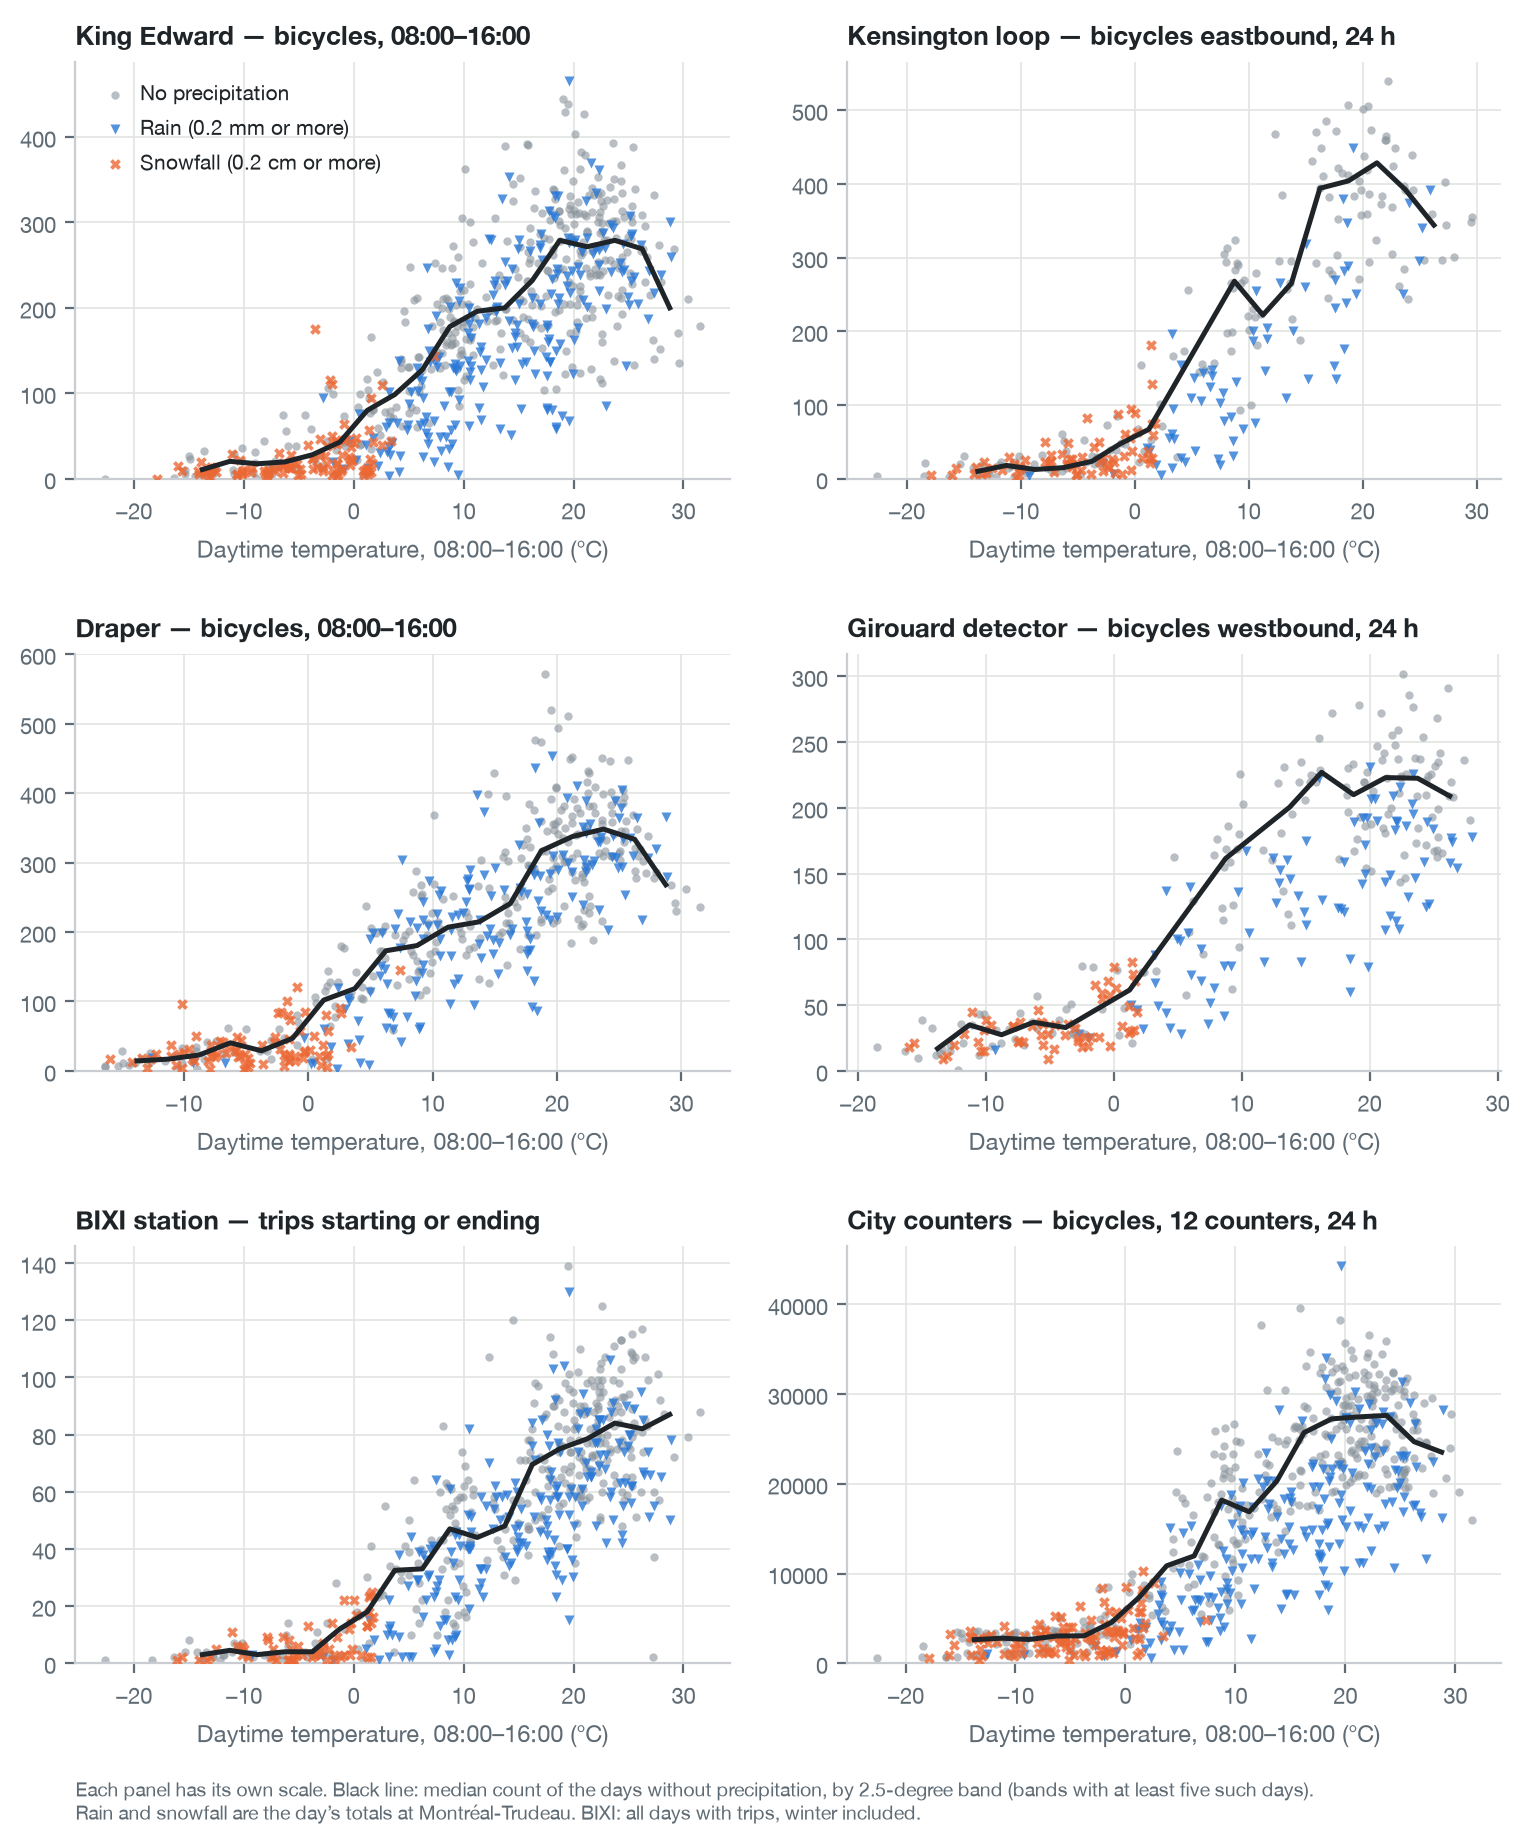
\includegraphics[width=0.95\textwidth]{../derived/figures/temperature-scatter/temperature_scatter_en.png}\caption{Daily count against daytime temperature, days marked by precipitation. Black line: median of the days without precipitation, by 2.5-degree band.}\label{fig:temperature_scatter}\end{figure}
Figure~\ref{fig:temperature_scatter} shows the raw relation. Figure~\ref{fig:temperature_curve} shows the fitted response with everything else held fixed, each series relative to its own level at 20\,$^\circ$C.
\begin{figure}[htbp]\centering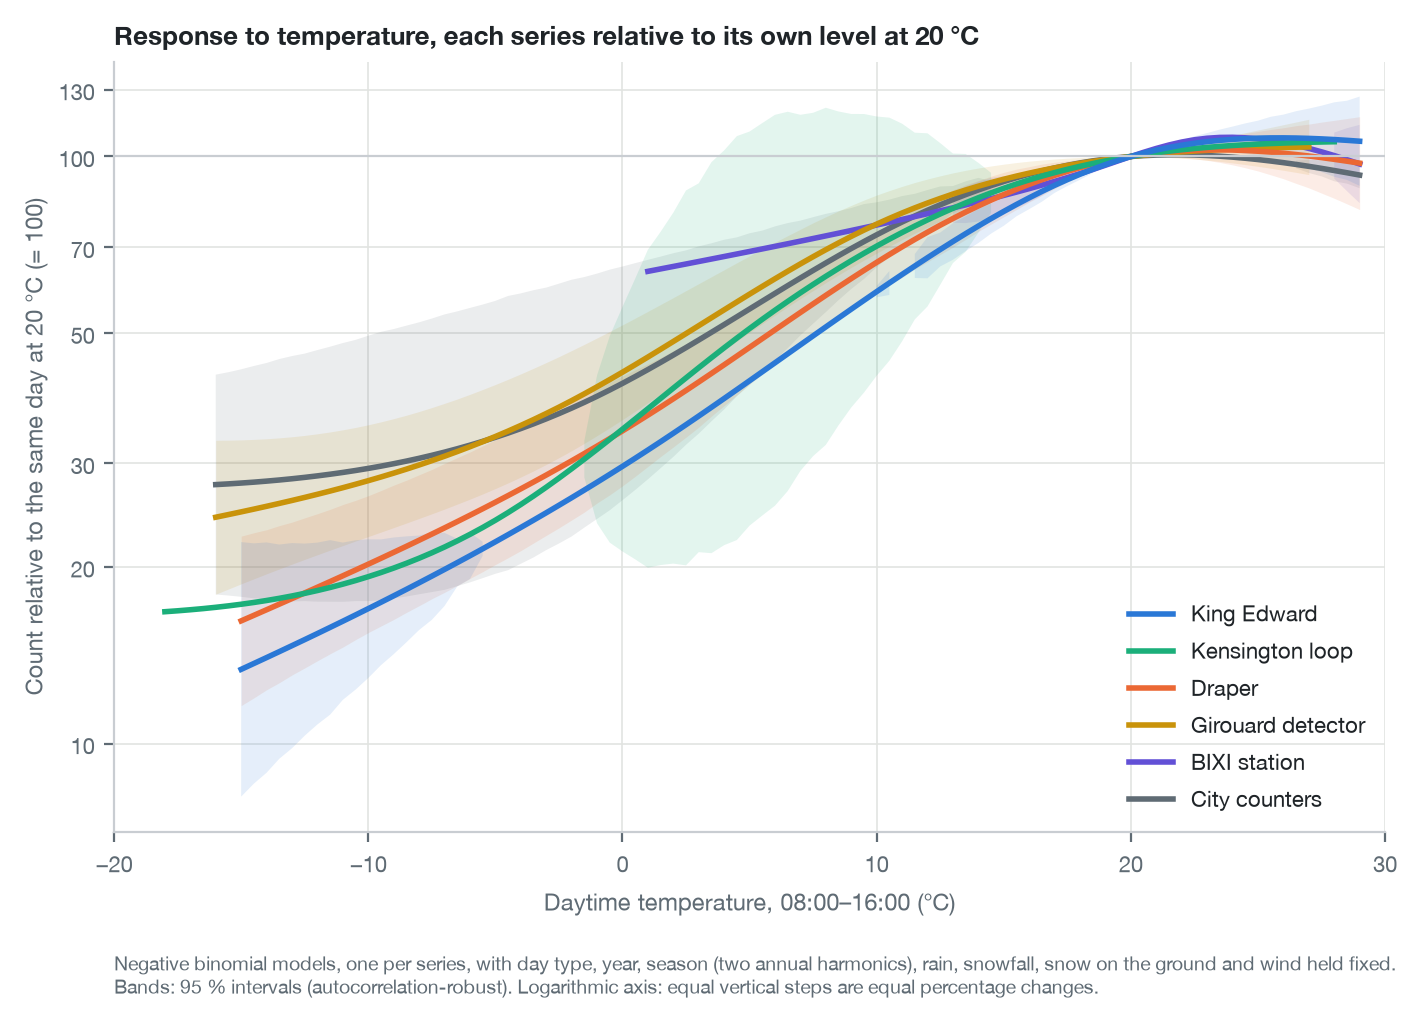
\includegraphics[width=0.85\textwidth]{../derived/figures/temperature-curve/temperature_curve_en.png}\caption{Fitted response to temperature (spline model), relative to 20\,$^\circ$C.}\label{fig:temperature_curve}\end{figure}
\begin{center}\small\begin{tabular}{@{}rrrrrrr@{}}\toprule
Daytime temperature ($^\circ$C) & King Edward & Kensington loop & Draper & Girouard detector & BIXI station & City counters\\\midrule
$-$15 & 13 & 17 & 16 & 25 & $-$$-$ & 28 \\
$-$10 & 17 & 19 & 20 & 28 & $-$$-$ & 29 \\
$-$5 & 22 & 24 & 26 & 33 & $-$$-$ & 33 \\
0 & 30 & 34 & 34 & 43 & $-$$-$ & 41 \\
5 & 41 & 51 & 47 & 58 & 69 & 55 \\
10 & 59 & 70 & 66 & 77 & 76 & 74 \\
15 & 81 & 88 & 86 & 91 & 86 & 91 \\
20 & 100 & 100 & 100 & 100 & 100 & 100 \\
25 & 107 & 105 & 102 & 103 & 107 & 99 \\
\bottomrule\multicolumn{7}{@{}l}{\footnotesize Count relative to the same day at 20\,$^\circ$C (= 100), spline model. BIXI: regular season only.}\end{tabular}\end{center}

\textbf{Slopes.} With temperature as a line with one change of slope:
\begin{center}\small\begin{tabular}{@{}lp{2.9cm}p{3.2cm}p{3.2cm}p{3.2cm}@{}}\toprule
Series & Change of slope, $^\circ$C (bootstrap 95\,\%) & Below it: \% per degree & Above it: \% per degree & Below it, within calendar months\\\midrule
King Edward & 20.0 (10 to 26) & +6.1 (+4.9 to +7.4) & +0.4 ($-$1.6 to +2.4) & +6.6 (+5.3 to +8.0) \\
Kensington loop & 18.0 (-8 to 26) & +5.6 (+4.5 to +6.8) & 0.0 ($-$2.1 to +2.2) & +6.3 (+5.1 to +7.4) \\
Draper & 24.5 (8 to 25) & +5.0 (+4.1 to +5.8) & $-$7.9 ($-$10.2 to $-$5.5) & +5.0 (+4.1 to +5.9) \\
Girouard detector & 15.5 (5 to 23) & +4.6 (+3.5 to +5.6) & +0.8 ($-$0.6 to +2.1) & +5.1 (+3.9 to +6.3) \\
BIXI station & 23.5 (1 to 26) & +2.7 (+1.9 to +3.4) & $-$2.2 ($-$5.5 to +1.2) & +3.2 (+2.5 to +3.9) \\
City counters & 20.5 (-3 to 24) & +3.7 (+3.1 to +4.4) & $-$1.7 ($-$3.0 to $-$0.4) & +4.4 (+3.8 to +5.0) \\
\bottomrule\end{tabular}\end{center}
On the four Terrebonne series each degree below the change of slope goes with 5 to 6\,\% more bicycles, and the estimate is the same when only days of the same calendar month are compared (last column). The BIXI station and the City counters show smaller slopes (2.7 and 3.7\,\%). Above the change of slope the count is flat or falls slightly.

\textbf{Where the slope changes.} The lowest deviance is at 20, 18, 24.5, 15.5\,$^\circ$C for King Edward, the Kensington loop, Draper and the Girouard detector, but the bootstrap intervals are wide (Appendix~\ref{app:bp}): the response bends gradually, as the spline shows, rather than at a point. The spline and the two-segment line fit about equally well (Appendix~\ref{app:aic}); a single straight line on the log scale fits worse on every series.

\textbf{Is there a second change in the cold?} Adding a change of slope at 0\,$^\circ$C to the model:
\begin{center}\small\begin{tabular}{@{}lrp{3.6cm}p{3.6cm}r@{}}\toprule
Series & Days below 0\,$^\circ$C & Below 0\,$^\circ$C: \% per degree & 0\,$^\circ$C to the change of slope: \% per degree & $p$ (difference)\\\midrule
King Edward & 135 & +5.2 (+1.9 to +8.6) & +6.5 (+5.5 to +7.6) & 0.47 \\
Kensington loop & 108 & +5.0 (+3.5 to +6.4) & +6.3 (+4.7 to +8.0) & 0.22 \\
Draper & 109 & +4.6 (+2.5 to +6.8) & +5.1 (+3.9 to +6.3) & 0.74 \\
Girouard detector & 87 & +4.0 (+2.3 to +5.8) & +5.3 (+3.7 to +6.8) & 0.36 \\
City counters & 169 & +2.4 (+1.4 to +3.5) & +4.8 (+3.9 to +5.6) & 0.00 \\
\bottomrule\end{tabular}\end{center}
On the Terrebonne series the two slopes are not distinguishable. The earlier analyses, which fitted two straight lines to the counts themselves, placed a change of slope at $-$1\,$^\circ$C (air temperature) or $-$5\,$^\circ$C (feels-like temperature): a count that falls by a constant percentage per degree traces a curve that flattens towards zero, and two straight lines fitted to that curve meet near where it flattens. The City counters do show a flatter slope below 0\,$^\circ$C.

\section{Wind chill}
The wind-chill index and the daytime temperature are almost the same variable over a year (correlation 0.996). A model with the wind-chill index in place of temperature and wind has an AIC that differs by $-$3.9 to +1.8 on the Terrebonne series (negative values favour wind chill; Appendix~\ref{app:aic}): small differences, three of four in its favour, not enough to say that riders respond to wind chill rather than to temperature. Wind as a separate term goes with $-$7 ($-$10 to $-$3)\,\% per 10\,km/h at King Edward and is not distinguishable from zero on the other three Terrebonne series.

\section{Rain, snow and wind}
\begin{figure}[htbp]\centering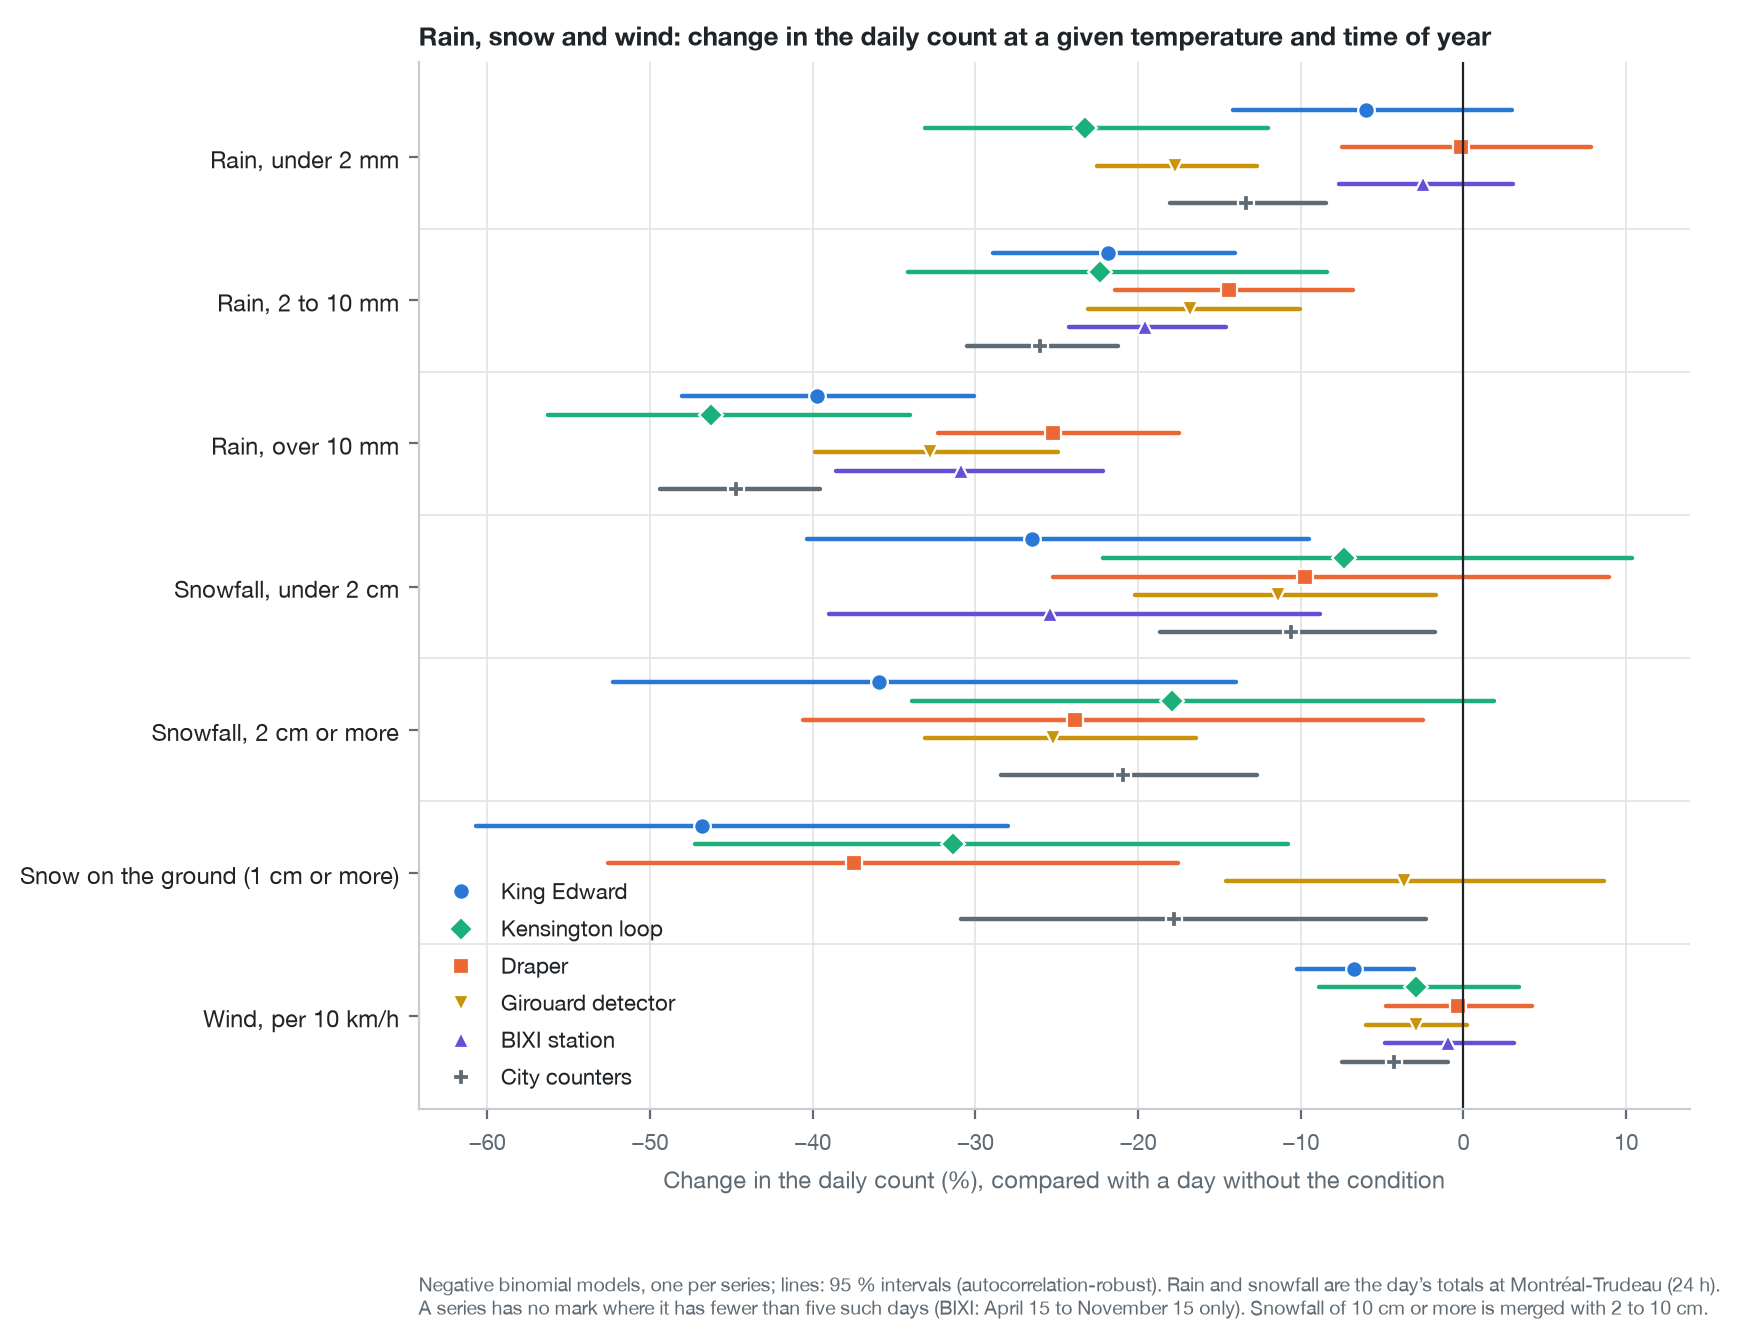
\includegraphics[width=0.92\textwidth]{../derived/figures/effects/effects_en.png}\caption{Change in the daily count associated with each condition, temperature and time of year held fixed.}\label{fig:effects}\end{figure}
\begin{center}\scriptsize\setlength{\tabcolsep}{3pt}\begin{tabular}{@{}lllllll@{}}\toprule
Condition & King Edward & Kensington loop & Draper & Girouard detector & BIXI station & City counters\\\midrule
Rain, under 2 mm & $-$6 ($-$14 to +3) & $-$23 ($-$33 to $-$12) & 0 ($-$7 to +8) & $-$18 ($-$23 to $-$13) & $-$2 ($-$8 to +3) & $-$13 ($-$18 to $-$8) \\
Rain, 2 to 10 mm & $-$22 ($-$29 to $-$14) & $-$22 ($-$34 to $-$8) & $-$14 ($-$21 to $-$7) & $-$17 ($-$23 to $-$10) & $-$20 ($-$24 to $-$15) & $-$26 ($-$31 to $-$21) \\
Rain, over 10 mm & $-$40 ($-$48 to $-$30) & $-$46 ($-$56 to $-$34) & $-$25 ($-$32 to $-$17) & $-$33 ($-$40 to $-$25) & $-$31 ($-$39 to $-$22) & $-$45 ($-$49 to $-$40) \\
Snowfall, under 2 cm & $-$27 ($-$40 to $-$9) & $-$7 ($-$22 to +10) & $-$10 ($-$25 to +9) & $-$11 ($-$20 to $-$2) & $-$25 ($-$39 to $-$9) & $-$11 ($-$19 to $-$2) \\
Snowfall, 2 cm or more & $-$36 ($-$52 to $-$14) & $-$18 ($-$34 to +2) & $-$24 ($-$41 to $-$2) & $-$25 ($-$33 to $-$16) & -- & $-$21 ($-$28 to $-$13) \\
Snow on the ground, 1 cm or more & $-$47 ($-$61 to $-$28) & $-$31 ($-$47 to $-$11) & $-$37 ($-$53 to $-$18) & $-$4 ($-$15 to +9) & -- & $-$18 ($-$31 to $-$2) \\
Wind, per 10 km/h & $-$7 ($-$10 to $-$3) & $-$3 ($-$9 to +3) & 0 ($-$5 to +4) & $-$3 ($-$6 to 0) & $-$1 ($-$5 to +3) & $-$4 ($-$7 to $-$1) \\
Snowfall the day before, per cm & $-$1 ($-$4 to +1) & $-$1 ($-$5 to +2) & $-$1 ($-$2 to +1) & $-$2 ($-$5 to +1) & $-$4 ($-$8 to 0) & $-$1 ($-$2 to 0) \\
Saturday & $-$8 ($-$16 to +1) & $-$34 ($-$42 to $-$24) & 0 ($-$9 to +9) & $-$22 ($-$27 to $-$18) & $-$11 ($-$16 to $-$5) & $-$36 ($-$41 to $-$31) \\
Sunday or holiday & $-$2 ($-$9 to +6) & $-$32 ($-$39 to $-$25) & +7 ($-$2 to +16) & $-$30 ($-$34 to $-$25) & $-$20 ($-$25 to $-$15) & $-$42 ($-$45 to $-$38) \\
December 24 to January 2 & $-$22 ($-$39 to 0) & $-$49 ($-$72 to $-$7) & $-$49 ($-$66 to $-$25) & $-$36 ($-$45 to $-$25) & -- & $-$62 ($-$68 to $-$55) \\
\bottomrule\multicolumn{7}{@{}p{16cm}}{\scriptsize Percentage change in the daily count (95\,\% interval), compared with a day without the condition (for the day types, with a weekday). --: fewer than five such days, or not applicable.}\end{tabular}\end{center}
Number of days behind each estimate:
\begin{center}\footnotesize\begin{tabular}{@{}p{4.6cm}rrrrrr@{}}\toprule
Condition & King Edward & Kensington loop & Draper & Girouard detector & BIXI station & City counters\\\midrule
Rain, under 2 mm & 81 & 25 & 61 & 33 & 58 & 77 \\
Rain, 2 to 10 mm & 110 & 37 & 76 & 40 & 79 & 92 \\
Rain, over 10 mm & 45 & 15 & 36 & 26 & 39 & 47 \\
Snowfall, under 2 cm & 56 & 38 & 48 & 30 & 9 & 64 \\
Snowfall, 2 cm or more & 46 & 30 & 30 & 26 & -- & 46 \\
Snow on the ground, 1 cm or more & 120 & 105 & 93 & 88 & -- & 161 \\
\bottomrule\end{tabular}\end{center}
Light rain (under 2\,mm in 24 hours) is not distinguishable from none on the camera sensors, which count 08:00--16:00; the two 24-hour counters on the street, the loop and the Girouard detector, show a reduction. Snow on the ground goes with a third to a half fewer bicycles at King Edward, Draper and Kensington and with no measurable change at the Girouard detector ($-$4 ($-$15 to +9)\,\%, 88 such days); the record does not say why the east end differs. The effects are multiplicative: on a January day that would see 20 bicycles in the window, 2 to 10\,mm of rain removes about four; on a June day that would see 300, about sixty. Snow on the ground carries the persistence of a snowfall: once it is in the model, the snowfall of the day before adds little.

\section{Day length, season and darkness}
\begin{figure}[htbp]\centering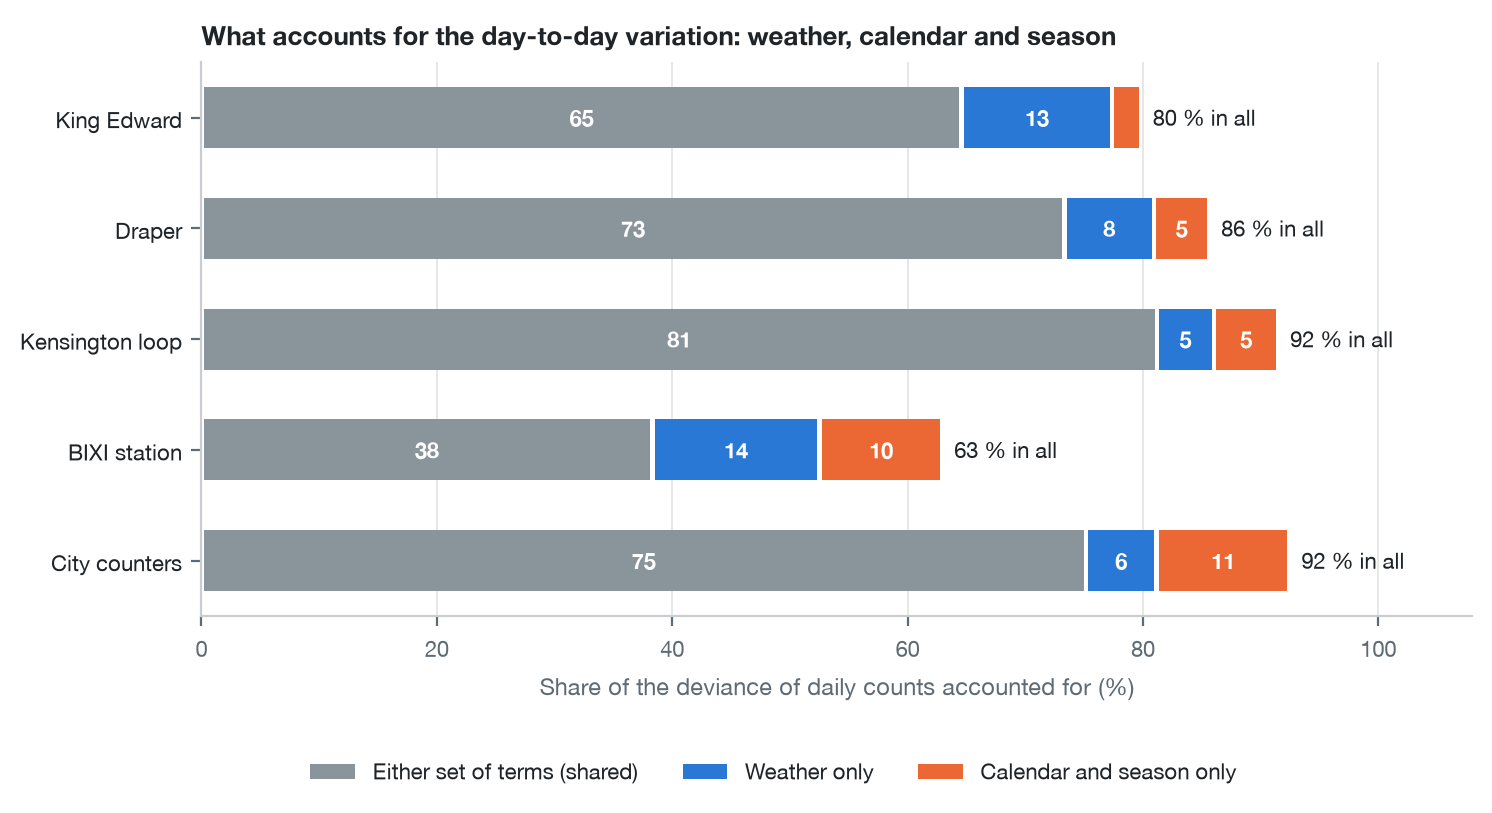
\includegraphics[width=0.85\textwidth]{../derived/figures/season-weather/season_weather_en.png}\caption{Share of the deviance of daily counts accounted for by the two sets of terms.}\label{fig:season_weather}\end{figure}
\begin{center}\footnotesize\begin{tabular}{@{}lrrrrrr@{}}\toprule
 & \multicolumn{3}{c}{Deviance accounted for (\%)} & \multicolumn{3}{c}{of which (\%)}\\\cmidrule(lr){2-4}\cmidrule(l){5-7}
Series & Calendar and season alone & Weather alone & Both & Either & Weather only & Calendar and season only\\\midrule
King Edward & 67 & 77 & 80 & 65 & 13 & 2 \\
Kensington loop & 87 & 86 & 92 & 81 & 5 & 5 \\
Draper & 78 & 81 & 86 & 73 & 8 & 5 \\
Girouard detector & 88 & 87 & 93 & 82 & 5 & 6 \\
BIXI station & 49 & 53 & 63 & 38 & 14 & 10 \\
City counters & 86 & 81 & 92 & 75 & 6 & 11 \\
\bottomrule\end{tabular}\end{center}
Most of what the models account for can be credited to either set of terms: the time of year predicts the weather, and the weather predicts the time of year. The record cannot say how much of the winter low is cold and snow and how much is the season as such. What it does say is that weather matters \emph{within} the season: the weather-only share is 5 to 13\,\% on the Terrebonne series, and the temperature slope is unchanged when estimated inside calendar months.

\begin{figure}[htbp]\centering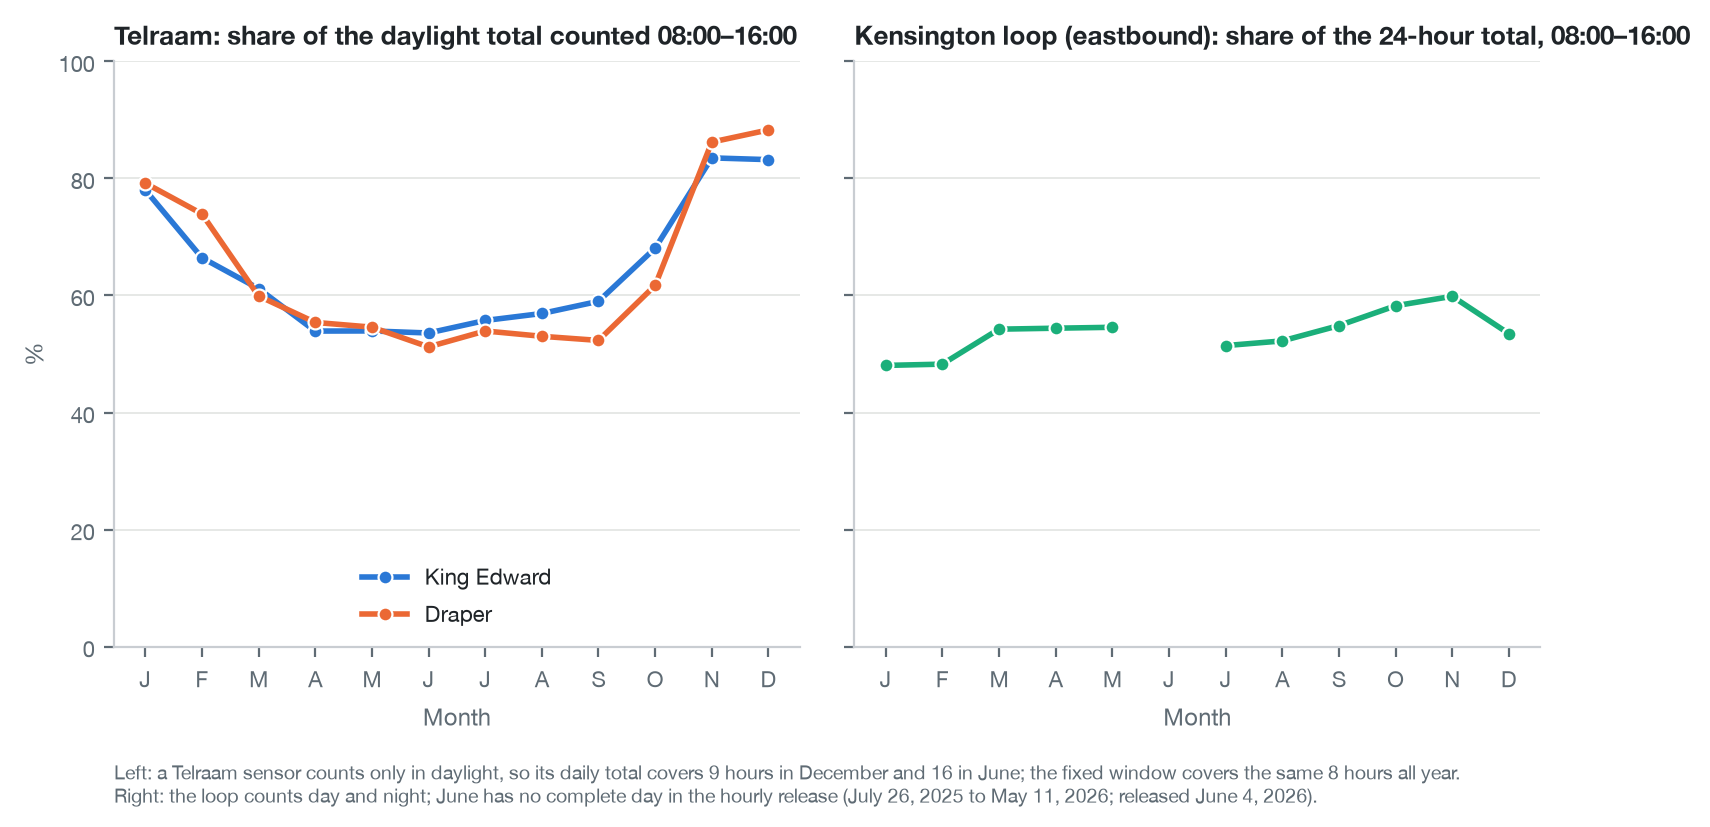
\includegraphics[width=0.95\textwidth]{../derived/figures/daylight/daylight_en.png}\caption{Left: the share of a Telraam sensor\textquoteright{}s daylight total that falls in the fixed window. Right: the share of the loop\textquoteright{}s 24-hour total in the same window.}\label{fig:daylight}\end{figure}
\textbf{What a daylight-only sensor sees.} In June the 08:00--16:00 window holds a little over half of a Telraam sensor\textquoteright{}s daily total; in December it holds more than 80\,\%, because there is little daylight outside it. A year-round comparison of Telraam daily totals therefore mixes a change in riding with a change in counting hours. On the loop, which counts day and night, the same window holds 46 to 57\,\% of the 24-hour total in every month of the hourly record, so the fixed window is a stable part of the day.

\textbf{Darkness at the same clock hour.} The loop\textquoteright{}s hourly record (4,592 hours between 06:00 and 22:00 on 287 days, 1,116 of them after sunset and 231 before sunrise) allows a direct comparison: the same hour of the same type of day, in the same month and at the same temperature, when the sun is up and when it is down. An evening hour after sunset carries 27\,\% (19 to 34) fewer bicycles, a morning hour before sunrise 17\,\% (3 to 30). In the same model an hour with rain observed carries 47\,\% (38 to 55) and an hour with snow observed 26\,\% (13 to 37). This is one site and one direction; with month constants in the model, the comparison rests mostly on the weeks around the clock changes and the equinoxes.

\section{Snowfall, the days after, and snow loading}
\begin{figure}[htbp]\centering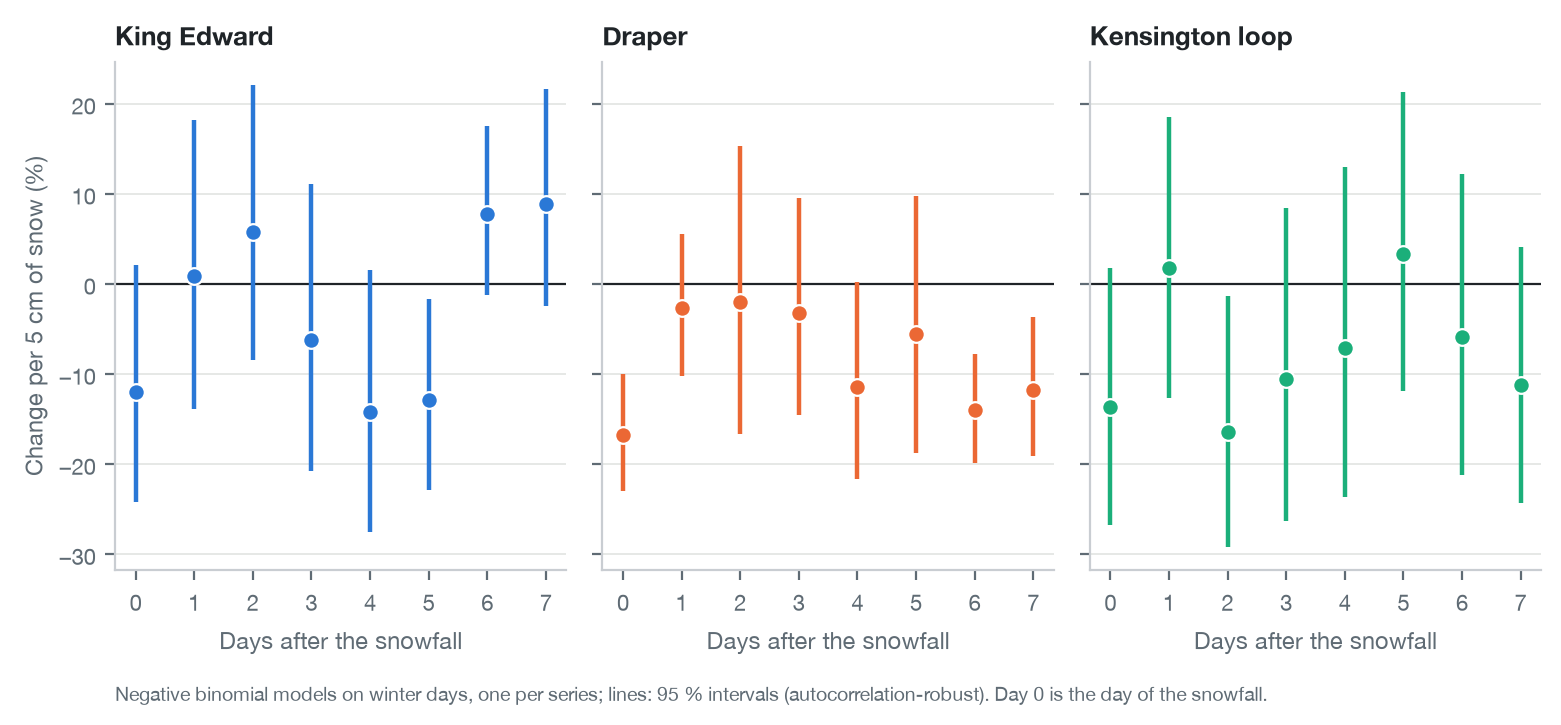
\includegraphics[width=0.95\textwidth]{../derived/figures/snow-lags/snow_lags_en.png}\caption{Winter days: change in the count per 5\,cm of snowfall on the day and on each of the seven days before.}\label{fig:snow_lags}\end{figure}
On winter days (November~16 to March~31), with temperature, rain, wind, day type and snow on the ground in the model:
\begin{center}\footnotesize\scriptsize\begin{tabular}{@{}rllll@{}}\toprule
Days after the snowfall & King Edward & Kensington loop & Draper & Girouard detector\\\midrule
0 & $-$12 ($-$24 to +2) & $-$14 ($-$27 to +2) & $-$17 ($-$23 to $-$9) & $-$13 ($-$22 to $-$3) \\
1 & +1 ($-$14 to +18) & +2 ($-$13 to +18) & $-$1 ($-$9 to +8) & +10 (+1 to +21) \\
2 & +6 ($-$8 to +22) & $-$16 ($-$29 to $-$1) & $-$2 ($-$17 to +15) & +8 ($-$7 to +25) \\
3 & $-$6 ($-$21 to +11) & $-$11 ($-$26 to +8) & $-$4 ($-$15 to +9) & +2 ($-$15 to +22) \\
4 & $-$14 ($-$28 to +2) & $-$7 ($-$24 to +13) & $-$13 ($-$22 to $-$2) & $-$3 ($-$15 to +10) \\
5 & $-$13 ($-$23 to $-$2) & +3 ($-$12 to +21) & $-$6 ($-$19 to +9) & +6 ($-$6 to +19) \\
6 & +8 ($-$1 to +18) & $-$6 ($-$21 to +12) & $-$14 ($-$20 to $-$9) & $-$2 ($-$9 to +6) \\
7 & +9 ($-$2 to +22) & $-$11 ($-$24 to +4) & $-$12 ($-$19 to $-$4) & +3 ($-$10 to +18) \\
\bottomrule\multicolumn{5}{@{}l}{\footnotesize Percentage change per 5\,cm of snow (95\,\% interval).}\end{tabular}\end{center}
The day of a snowfall shows the clearest reduction (12 to 17\,\% per 5\,cm; the interval excludes zero at Draper and the Girouard detector). On the following days the estimates scatter around zero and a few negative values, with wide intervals and no pattern common to the four series; winter counts are small (a few dozen a day), each series has 109 to 191 winter days, and snow on the ground already carries part of the after-effect. An average over snowfall episodes was also computed (\texttt{snow\_episodes\_summary.csv}); with fewer than ten episodes of 10\,cm or more per series it is too noisy to read.

\textbf{Snow-loading days.}
\begin{center}\small\begin{tabular}{@{}llrrp{3.4cm}p{3.4cm}@{}}\toprule
Series & Sector & Winter days & of which loading days & Loading day: change (\%) & Temperature: \% per degree (winter only)\\\midrule
King Edward & CDN-301 & 191 & 44 & $-$4 ($-$29 to +30) & +7 (+5 to +9) \\
Kensington loop & CDN-301 & 132 & 36 & +2 ($-$25 to +39) & +7 (+5 to +10) \\
Draper & CDN-111 & 154 & 34 & $-$18 ($-$45 to +22) & +7 (+5 to +9) \\
Girouard detector & CDN-111 & 109 & 18 & $-$9 ($-$25 to +11) & +4 (+2 to +6) \\
\bottomrule\end{tabular}\end{center}
On the days the City loaded snow in the sector that contains the counter, the counts are not distinguishable from those of other winter days with the same temperature and snow. The intervals are wide enough to contain a reduction of a quarter or more as well as no change; the record does not settle the question. In winter alone, each degree goes with 4 to 7\,\% more bicycles on the four series.

\section{Location: what differs along the street}\label{sec:location}
The counters do not measure the same thing at the same place, and none of the differences between them is a discrepancy. The street runs from a more residential west end towards downtown; a counter further east can be expected to see more through traffic and more commuters, and the resident population around the counters also differs:
\begin{center}\footnotesize\resizebox{\textwidth}{!}{\begin{tabular}{@{}lrrrrll@{}}\toprule
Counter (west to east) & From the west end (km) & To downtown (km) & Residents within 500\,m & Residents per km$^2$ & Motor traffic & Instrument\\\midrule
King Edward & 0.48 & 6.7 & 6,130 & 7,800 & one-way westbound & camera sensor, 08:00--16:00 \\
Kensington loop & 1.35 & 5.9 & 5,760 & 7,300 & one-way eastbound & loop, 24 h \\
BIXI station & 1.40 & 5.9 & 5,730 & 7,300 & one-way eastbound & bike-share dock \\
Draper & 1.85 & 5.4 & 6,890 & 8,800 & one-way eastbound & camera sensor, 08:00--16:00 \\
Girouard detector & 2.41 & 4.9 & 9,320 & 11,900 & one-way eastbound & detector, 24 h \\
\bottomrule\multicolumn{7}{@{}p{16cm}}{\footnotesize Distances in a straight line, the first from the west end of the lane; downtown reference point: avenue McGill College at rue Sainte-Catherine Ouest. Residents: 2021 Census, dissemination areas, weighted by the share of each area within 500\,m of the counter (Statistics Canada).}\end{tabular}}\end{center}
\textbf{What location can and cannot be adjusted for.} Each counter is its own location in every model of this note, with its own level and its own responses. An adjustment for « centrality » as such, a coefficient for distance to downtown or for population density, cannot be estimated from this record: there are four counters on the street, of three different kinds (two camera sensors read over eight daytime hours in both directions, one loop and one detector counting 24 hours in one direction each), so position and instrument cannot be told apart, and four points do not determine a gradient. The table above gives the context in which each counter\textquoteright{}s figures are to be read.

\textbf{The one like-for-like comparison of two locations.} The two camera sensors are the same instrument, read in the same window. On the days valid at both:
\begin{center}\small\resizebox{\textwidth}{!}{\begin{tabular}{@{}lrrrl@{}}\toprule
Days & Number & King Edward, mean a day & Draper, mean a day & Draper over King Edward (95\,\% interval)\\\midrule
all days valid at both & 456 & 164 & 201 & 1.22 (1.16 to 1.29) \\
winter (Nov 16 -- Mar 31) & 129 & 36 & 51 & 1.43 (1.07 to 1.73) \\
rest of the year & 327 & 215 & 260 & 1.21 (1.15 to 1.28) \\
weekdays & 314 & 166 & 198 & 1.20 (1.12 to 1.29) \\
Saturdays, Sundays, holidays & 142 & 162 & 207 & 1.28 (1.20 to 1.38) \\
\bottomrule\end{tabular}}\end{center}
Draper, 1.4\,km further east, counts about a fifth more than King Edward in the same eight hours, and proportionately more in winter (the winter interval is wide). This is a difference between two places on the street.

\textbf{Do the effects differ by location?} A single model of the four counters on the street (1,780 counter-days), with a location term and its interaction with every other term, and standard errors clustered by date because the counters share each day\textquoteright{}s weather, tests whether each effect is the same at the four locations:
\begin{center}\small\begin{tabular}{@{}lrrrrrrr@{}}\toprule
 & \multicolumn{4}{c}{Effect at each location (\%)} & \multicolumn{3}{c}{Same at all four?}\\\cmidrule(lr){2-5}\cmidrule(l){6-8}
Term & King Edward & Kensington & Draper & Girouard & $\chi^2$ & df & $p$\\\midrule
temperature below 20\,$^\circ$C (per degree) & +6.1 & +5.5 & +5.4 & +4.1 & 7.7 & 3 & 0.053 \\
temperature above 20\,$^\circ$C (per degree) & +0.4 & $-$1.2 & $-$0.6 & 0.0 & 3.0 & 3 & 0.388 \\
rain, under 2 mm & $-$6 & $-$23 & $-$1 & $-$16 & 17.4 & 3 & $<$0.001 \\
rain, 2 to 10 mm & $-$22 & $-$22 & $-$14 & $-$16 & 4.4 & 3 & 0.220 \\
rain, over 10 mm & $-$40 & $-$46 & $-$25 & $-$31 & 13.9 & 3 & 0.003 \\
snowfall, under 2 cm & $-$26 & $-$8 & $-$9 & $-$12 & 4.2 & 3 & 0.240 \\
snowfall, 2 cm or more & $-$36 & $-$18 & $-$23 & $-$26 & 2.1 & 3 & 0.562 \\
snow on the ground & $-$47 & $-$31 & $-$38 & $-$4 & 28.3 & 3 & $<$0.001 \\
wind (per 10 km/h) & $-$7 & $-$3 & $-$1 & $-$3 & 3.2 & 3 & 0.361 \\
Saturday & $-$8 & $-$33 & $-$1 & $-$23 & 32.9 & 3 & $<$0.001 \\
Sunday or holiday & $-$2 & $-$32 & +6 & $-$30 & 96.8 & 3 & $<$0.001 \\
time of year (four harmonic terms) & -- & -- & -- & -- & 115.9 & 12 & $<$0.001 \\
\bottomrule\multicolumn{8}{@{}p{15.5cm}}{\footnotesize Change of slope fixed at 20\,$^\circ$C in this model so that the slopes are comparable. A small $p$ means the effect differs by location.}\end{tabular}\end{center}
The response to temperature below 20\,$^\circ$C is close along the street, a little steeper at the west end than at the east end (6.1 against 4.1\,\% per degree; the test is borderline). The effects that clearly differ are those of the weekend, of light and heavy rain, and of snow on the ground. The weekend and light-rain differences follow the instrument: the two 24-hour counters (the loop and the Girouard detector) show them and the two camera sensors, read 08:00--16:00, do not. Snow on the ground goes with a large reduction at King Edward, Kensington and Draper and with none at Girouard, at the east end. The record cannot say how much of any of this is the place and how much the instrument.

The BIXI station and the City\textquoteright{}s counters elsewhere respond less steeply to temperature than the counters on the street; they are different quantities again (trips at a dock; a sum of counters on other streets) and are shown for context.

\section{Year to year, after weather}
\textbf{Is the weather of each year allowed for?} Yes. The year term is estimated in the same model as temperature, rain, snowfall, snow on the ground and wind. A year that was colder, wetter or snowier is therefore compared with what the model expects for that weather, not with the raw count of a milder year. To make the part played by the weather visible, the comparison is shown here in three steps:
\begin{enumerate}
\item \emph{Plain comparison, no model:} the same calendar dates, valid in both years; the ratio of the two totals. It accounts for downtime (a date enters only if both years have it) but not for the weather.
\item \emph{Model with day type and time of year only,} no weather term.
\item \emph{The main model,} with the weather terms: the figure quoted in this note.
\end{enumerate}
\begin{center}\footnotesize\begin{tabular}{@{}llrlll@{}}\toprule
Series & Counting years & Dates in both & 1. Plain, same dates (\%) & 2. Season only (\%) & 3. With weather (\%)\\\midrule
King Edward & 2025--26 against 2024--25 & 254 & $-$5 ($-$16 to +4) & $-$12 ($-$23 to +1) & $-$1 ($-$11 to +9) \\
King Edward & 2026--27 against 2024--25 & 76 & +26 ($-$1 to +62) & +22 ($-$3 to +54) & +27 (+12 to +45) \\
Draper & 2025--26 against 2024--25 & 132 & $-$11 ($-$22 to $-$2) & $-$20 ($-$29 to $-$10) & $-$12 ($-$20 to $-$5) \\
City counters & 2025--26 against 2024--25 & 213 & $-$8 ($-$16 to +1) & $-$10 ($-$18 to $-$2) & $-$7 ($-$14 to 0) \\
\bottomrule\multicolumn{6}{@{}p{15.5cm}}{\footnotesize Counting years run from August 15. 95\,\% intervals: step 1, bootstrap over 14-day blocks of dates; steps 2 and 3, autocorrelation-robust. Comparisons with fewer than 30 dates in both years are not shown.}\end{tabular}\end{center}
How the weather differed, on the dates both years have (first year / later year):
\begin{center}\footnotesize\resizebox{\textwidth}{!}{\begin{tabular}{@{}lrrrrr@{}}\toprule
Comparison & Daytime temp. ($^\circ$C) & Days below $-$10\,$^\circ$C & Snowfall (cm) & Days, snow on ground & Rain (mm)\\\midrule
King Edward, 2025--26 against 2024--25 & 11.3 / 9.9 & 7 / 14 & 55 / 135 & 26 / 45 & 561 / 651 \\
King Edward, 2026--27 against 2024--25 & 15.9 / 15.3 & 0 / 0 & 0 / 0 & 0 / 0 & 150 / 212 \\
Draper, 2025--26 against 2024--25 & 12.9 / 12.0 & 5 / 7 & 13 / 22 & 14 / 21 & 236 / 398 \\
City counters, 2025--26 against 2024--25 & 9.9 / 9.0 & 19 / 26 & 88 / 111 & 53 / 65 & 454 / 551 \\
\bottomrule\end{tabular}}\end{center}
The weather matters to the answer. On the dates King Edward has in both of its first two years, the second year was colder (9.9 against 11.3\,$^\circ$C by day) and much snowier (135 against 55\,cm of snow, 45 against 26 days with snow on the ground). Compared plainly, the second year is $-$5 ($-$16 to +4)\,\%; with the time of year alone, $-$12 ($-$23 to +1)\,\%; once the weather is in the model, $-$1 ($-$11 to +9)\,\%: what looked like a lower second year is accounted for by a harder winter. At Draper the difference narrows with the weather but remains ($-$20 ($-$29 to $-$10) to $-$12 ($-$20 to $-$5)\,\%). King Edward\textquoteright{}s autumn of 2026 is higher than its autumn of 2024 at every step (+26 ($-$1 to +62)\,\% plainly, +27 (+12 to +45)\,\% with the weather); the two autumns were close in temperature (15.3 against 15.9\,$^\circ$C by day) and the autumn of 2026 had more rain (212 against 150\,mm).

The adjustment has its own limits: it assumes that riders respond to a given temperature or snowfall in the same way each year, the weather is measured at the airport, and the state of the lane itself (cleared or not) is not observed.

The year terms of the main model, for every series that has them:
\begin{center}\small\begin{tabular}{@{}llrp{4.2cm}@{}}\toprule
Series & Counting years (from August 15) & Days in the later year & Change (\%, 95\,\% interval)\\\midrule
King Edward & 2025--26 against 2024--25 & 272 & $-$1 ($-$11 to +9) \\
King Edward & 2026--27 against 2024--25 & 86 & +27 (+12 to +45) \\
Draper & 2025--26 against 2024--25 & 245 & $-$12 ($-$20 to $-$5) \\
BIXI station & 2025--26 against 2024--25 & 229 & $-$10 ($-$16 to $-$4) \\
City counters & 2025--26 against 2024--25 & 361 & $-$7 ($-$14 to 0) \\
\bottomrule\end{tabular}\end{center}
These figures are to be read with care. \textbf{Downtime is accounted for:} only days with a complete, valid count enter the models, nothing is filled in, and the year term compares each day with days of the same time of year, day type and weather. A month missing in one year therefore is not read as a decline; it simply contributes no days, and the year term rests on the months that year does have (on the model\textquoteright{}s assumption that the seasonal pattern is the same from year to year). What a year term cannot exclude is anything else that differs between the years: a camera sensor\textquoteright{}s field of view can change when it is remounted, and the 2026--27 counting year so far holds only August~15 to early November. King Edward\textquoteright{}s 2026--27 figure compares that autumn with the autumn of 2024. Draper\textquoteright{}s and the BIXI station\textquoteright{}s later years are merged (too few days after August~15, 2026), and the City counters\textquoteright{} 2026--27 term is not shown (its first year holds no autumn to compare with). The loop and the Girouard detector each have about one year and no such term.

\section{How well the models predict}
Each calendar month in turn was left out, the model fitted on the rest, and the month predicted:
\begin{center}\small\begin{tabular}{@{}lrrrrr@{}}\toprule
 & & \multicolumn{2}{c}{Median absolute error (\%)} & \multicolumn{2}{c}{$R^2$ on the log scale}\\\cmidrule(lr){3-4}\cmidrule(l){5-6}
Series & Days predicted & Fitted & Month left out & Fitted & Month left out\\\midrule
King Edward & 691 & 22 & 23 & 0.84 & 0.82 \\
Kensington loop & 284 & 20 & 25 & 0.92 & 0.87 \\
Draper & 505 & 19 & 20 & 0.88 & 0.86 \\
Girouard detector & 296 & 13 & 14 & 0.92 & 0.90 \\
BIXI station & 441 & 15 & 17 & 0.59 & 0.50 \\
City counters & 661 & 15 & 18 & 0.94 & 0.93 \\
\bottomrule\end{tabular}\end{center}
The typical day is predicted to within about a fifth to a quarter of its count, and little accuracy is lost on a month the model has not seen. A fifth of a small winter count is a few bicycles.

\section{Limits}
\begin{itemize}
\item \textbf{Daylight-only sensors.} The Telraam figures are 08:00--16:00 counts. They say nothing about evening and night riding, and their levels are never to be compared with the loop\textquoteright{}s.
\item \textbf{Gaps (accounted for, not filled).} Only complete, valid days are used and each is compared with like days, so downtime does not bias the estimates; it does reduce the days available. King Edward has no valid day in February 2026 and few in December 2025 and July 2026; Draper has none from February to April 2026. The winter of 2025--26 is therefore thinly covered by the camera sensors and carried mostly by the loop and the Girouard detector.
\item \textbf{The Girouard detector: one direction, one winter,} and a camera-type detector whose counting method the City\textquoteright{}s page does not detail.
\item \textbf{One loop site, one winter, one direction} in the models; the westbound channel is not used after the fault of March 2026, and for consistency not before.
\item \textbf{Weather at the airport,} 9\,km away; precipitation as 24-hour totals; the state of the lane itself (cleared or not, icy or not) is not observed. Snow on the ground at the airport stands in for it.
\item \textbf{Season and weather are confounded} and no model can fully separate them from this record.
\item \textbf{Association, not cause.} A percentage per degree describes days in the record; it does not predict what would happen under conditions the record does not contain.
\item \textbf{Uptime.} Telraam hours with an uptime under 0.5 are dropped; whether the remaining counts are already scaled for uptime is not documented.
\end{itemize}

\appendix
\section{Valid days by month}\label{app:coverage}
\begin{center}\footnotesize\begin{tabular}{@{}lrrrrrr@{}}\toprule
Month & King Edward & Kensington loop & Draper & Girouard detector & BIXI station & City counters\\\midrule
2024-08 & 14 & 0 & 0 & 0 & 31 & 0 \\
2024-09 & 26 & 0 & 4 & 0 & 30 & 0 \\
2024-10 & 28 & 0 & 18 & 0 & 31 & 0 \\
2024-11 & 29 & 0 & 21 & 0 & 21 & 0 \\
2024-12 & 19 & 0 & 21 & 0 & 0 & 0 \\
2025-01 & 26 & 0 & 24 & 0 & 0 & 30 \\
2025-02 & 27 & 0 & 22 & 0 & 0 & 21 \\
2025-03 & 30 & 0 & 22 & 0 & 0 & 30 \\
2025-04 & 30 & 0 & 30 & 0 & 20 & 30 \\
2025-05 & 31 & 0 & 29 & 0 & 31 & 31 \\
2025-06 & 30 & 0 & 30 & 0 & 30 & 30 \\
2025-07 & 31 & 6 & 30 & 0 & 29 & 31 \\
2025-08 & 30 & 31 & 27 & 0 & 14 & 31 \\
2025-09 & 28 & 30 & 28 & 0 & 30 & 30 \\
2025-10 & 31 & 31 & 31 & 8 & 31 & 31 \\
2025-11 & 30 & 30 & 27 & 30 & 30 & 30 \\
2025-12 & 14 & 31 & 26 & 31 & 31 & 31 \\
2026-01 & 25 & 29 & 12 & 19 & 25 & 29 \\
2026-02 & 0 & 28 & 0 & 26 & 23 & 28 \\
2026-03 & 22 & 29 & 0 & 18 & 28 & 29 \\
2026-04 & 30 & 30 & 0 & 6 & 30 & 30 \\
2026-05 & 31 & 28 & 18 & 25 & 31 & 31 \\
2026-06 & 29 & 27 & 25 & 30 & 30 & 30 \\
2026-07 & 10 & 31 & 19 & 27 & 31 & 31 \\
2026-08 & 22 & 31 & 16 & 31 & 31 & 31 \\
2026-09 & 30 & 0 & 17 & 30 & 0 & 30 \\
2026-10 & 31 & 0 & 13 & 15 & 0 & 31 \\
2026-11 & 8 & 0 & 0 & 0 & 0 & 6 \\
\bottomrule\multicolumn{7}{@{}p{12cm}}{\footnotesize Loop: days valid in the daily table (both directions); the models use the eastbound channel, to May~10, 2026. BIXI: days with at least one trip.}\end{tabular}\end{center}

\section{Model comparison}\label{app:aic}
\begin{center}\small\begin{tabular}{@{}lrrrrrr@{}}\toprule
 & \multicolumn{3}{c}{AIC, temperature as} & \multicolumn{2}{c}{AIC, without the wind term} & \\\cmidrule(lr){2-4}\cmidrule(lr){5-6}
Series & one line & two segments & spline & temperature & wind chill & Correlation, temperature and wind chill\\\midrule
King Edward & 7286.8 & 7269.8 & 7273.0 & 7276.2 & 7265.9 & 0.996 \\
Kensington loop & 2743.3 & 2734.9 & 2734.5 & 2733.8 & 2732.2 & 0.995 \\
Draper & 5413.0 & 5384.9 & 5389.1 & 5383.0 & 5381.2 & 0.996 \\
Girouard detector & 2630.2 & 2611.6 & 2610.9 & 2612.4 & 2613.4 & 0.997 \\
BIXI station & 3687.1 & 3676.5 & 3683.0 & 3674.8 & 3674.3 & 0.995 \\
City counters & 12286.9 & 12242.5 & 12218.5 & 12249.8 & 12237.4 & 0.996 \\
\bottomrule\end{tabular}\end{center}
Lower is better; differences of less than about 2 are not meaningful. AIC values are comparable only within a row.

\section{Where the slope changes: deviance profile}\label{app:bp}
\begin{figure}[H]\centering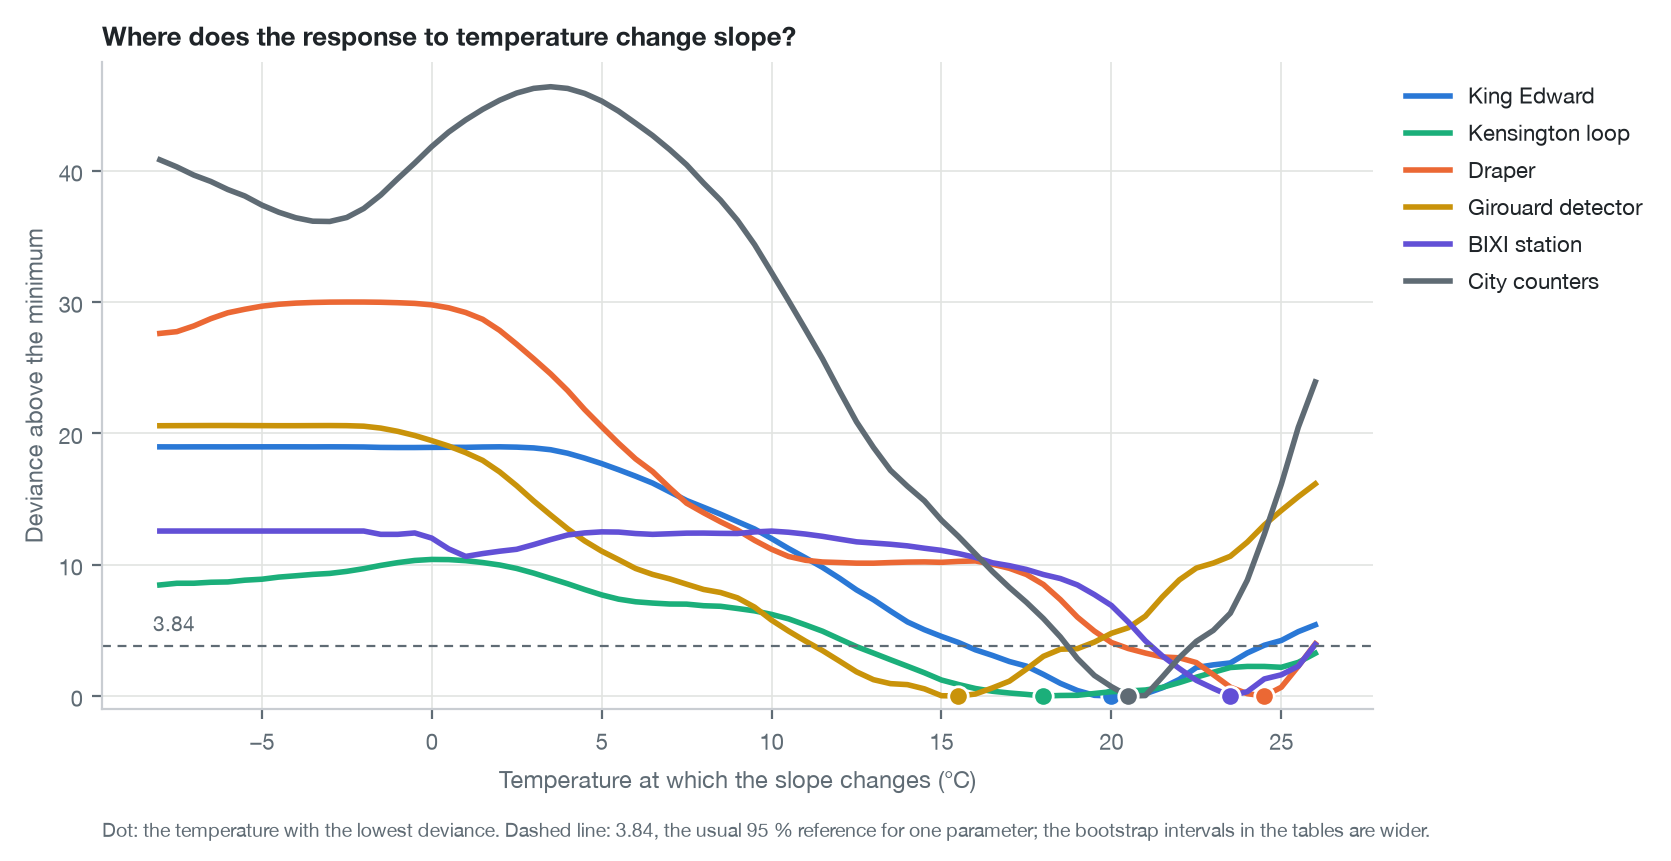
\includegraphics[width=0.85\textwidth]{../derived/figures/breakpoint/breakpoint_en.png}\caption{Deviance of the two-segment model as the change of slope is moved, each series relative to its own minimum.}\label{fig:breakpoint}\end{figure}

\section{The earlier analyses and what was kept}\label{app:matlab}
Between September 2024 and May 2026 the author explored the Telraam counts in MATLAB. Those scripts were read before this work; none of their code is used here. In summary:
\begin{center}\footnotesize\begin{tabular}{@{}p{3.3cm}p{6.6cm}p{5.6cm}@{}}\toprule
Earlier analysis & What it did & Here\\\midrule
Regressions of February 2025 & Least-squares fits of daily counts on temperature or feels-like temperature, squared terms, precipitation; two straight lines with a change of slope found by search ($-$1 and $-$5\,$^\circ$C); King Edward only, 290 days & Count model on the percentage scale; change of slope estimated with an interval, segments joined; the cold change of slope tested and not found \\
Sunset adjustment & Counts up to 15:00 multiplied by a fixed ratio (1.65 on weekdays, 1.37 on weekends) to stand for the whole day & Replaced by the fixed 08:00--16:00 window, with no scaling \\
Filling of dark hours & Five ways to fill the hours after sunset from a reference daily profile & Not kept: no count is estimated for hours the sensor did not see \\
Daily weather regression of November 2025 & Least squares on before-15:00 counts with temperature, precipitation, wind, weekend and a linear trend; ten interaction tests; weather classes compared by $t$-tests & Kept as the main model, with a count distribution, season terms in place of the trend and autocorrelation-robust intervals \\
Weekly season-and-anomaly split & Share of variance from a seasonal baseline and from weather anomalies, weekly & Kept, daily, as the deviance shares and the within-month model \\
Lagged-snow regression and snow-event averages, winter 2024--25 & Ten lags of a snow proxy (precipitation on days below 0\,$^\circ$C); average response by snowfall class & Kept with measured snowfall and snow on the ground, two winters, four series, and the City\textquoteright{}s loading record \\
Winter retention, storm recovery, composite scores & Ratios of winter to summer counts by mode; one storm; ad hoc scores & Not kept \\
Weather source & A commercial city-level feed & Environment and Climate Change Canada, Montréal-Trudeau \\
\bottomrule\end{tabular}\end{center}

\section{Sources}
Environment and Climate Change Canada, historical climate data, MONTREAL INTL A (7025251), downloaded November~10, 2026. Telraam (citizen-operated sensors; the counts belong to Telraam). Arrondissement de Côte-des-Neiges--Notre-Dame-de-Grâce, loop counter at Terrebonne/Kensington, access requests 2026-300 (released June~4, 2026) and 2026-581 (released October~9, 2026). Ville de Montréal open data: permanent bicycle counters (files of November~7, 2026), snow-removal transactions; CC~BY~4.0. BIXI Montréal open data, trip history 2024--2026 (downloaded November~10, 2026; listed by the City\textquoteright{}s portal under CC~BY~4.0, attribution to BIXI Montréal). Details and licences: the folder\textquoteright{}s README.
\end{document}
